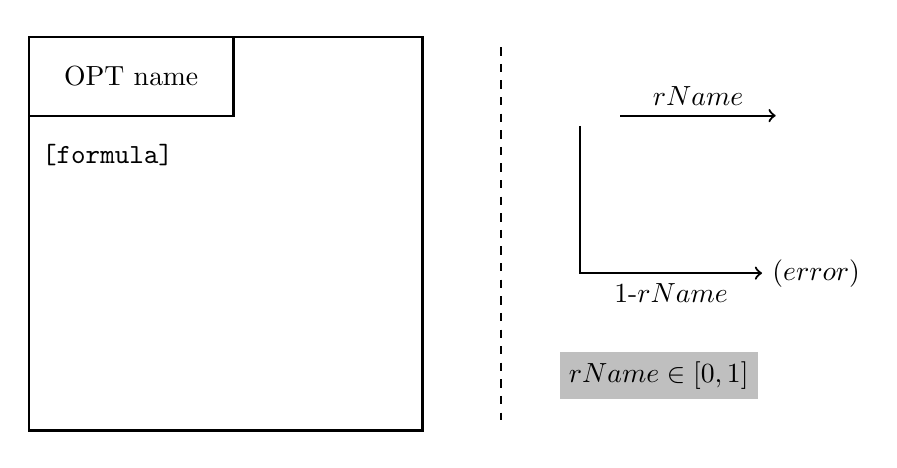
\begin{tikzpicture}[thick]
%%%%%%%%%%%%%%%%%%%%%%%%%%%%%%%%%%%%%%%%%%% HELP LINES
%\draw[help lines] (0,0) grid +(10,10);

%%%%%%%%%%%%%%%%%%%%%%%%%%%%%%%%%%%%%%%%%%% elements
\draw (1,0) rectangle +(5,5);

%%%%% guards and constraints
\node[shape=rectangle, draw=black, minimum height=1cm, minimum width=2.6cm](alt)at(2.3,4.5){OPT name};
\node[shape=rectangle, draw=none](guard) at (2,3.5) {\texttt{[formula]}};

\node[transparent](t1) at (7,5){};
\node[transparent](t2) at (7,0){};
\draw[dashed] (t1) -- (t2);

\node[dashed, minimum width=1cm](current) at (8,4){};
\node[dashed, minimum width=1cm](error) at (11,2){($error$)};
\node[ minimum width=1cm](regular) at (11,4){};
\node[rectangle, draw=none, fill=gray!50](constraint) at (9,0.7){$rName \in [0,1]$};

\draw[->,thick] (current.east) -- node[draw=none, rectangle, above]{$rName$}(regular.west);
\draw[->,thick] (current.south) |- node[draw=none, rectangle, near end, below]{1-$rName$}(error.west);
\end{tikzpicture}
